
\subsubsection{5.1 Oracle Isolation Gap (RQ1)}

\textbf{Table 1: Oracle Isolation Gate Metrics (Experiment A)}

\begin{table}[htbp]
\centering
\resizebox{\columnwidth}{!}{%
\begin{tabular}{llll}
\toprule
Metric & Value & Threshold & Status \\
\midrule
Mean oracle-isolation gap & **0.4012** & $\geq$ 0.10 & PASS ($4\times )$ \\
95\% CI & [0.358, 0.445] & --- & --- \\
Wilcoxon p (Holm-corrected) & **5.88e-38** & < 0.01 & PASS \\
Mean contract-unique (CU) mass & **0.4023** & $\geq$ 0.05 & PASS ($8\times )$ \\
CU mass 95\% CI lower & 0.360 & > 0.03 & PASS \\
Task coverage & 364 / 364 (100\%) & $\geq$ 90\% & PASS \\
\bottomrule
\end{tabular}
}
\end{table}

Source: \texttt{h-m1/code/results/oracle\textbackslash \_isolation\textbackslash \_results.json}

The contract oracle detects failures on 40.1\% more triples than the differential oracle on CVT inputs. The mean differential failure rate is 0.596 and the mean contract failure rate is 0.997 on CVT inputs. The near-unity contract failure rate is expected by construction: CVTs are specifically selected to trigger contract violations, so the reference contract oracle fires on essentially all of them. The scientifically informative quantity is the contract-unique mass (0.40): among evaluations where the LLM program matches the reference output (Oracle A: PASS), the contract oracle identifies 40\% as semantically invalid. These programs produce the correct-looking output on a contract-violating input while the reference contract asserts the behavior is invalid --- a class of error that differential equality testing cannot detect, regardless of test count.

\textbf{Stratification by task type:} HumanEval+ tasks (n = 117) show a mean gap of 0.520; MBPP+ tasks (n = 247) show a mean gap of 0.345, indicating a systematic task-type effect. HumanEval+ contracts appear to more frequently enforce relational invariants that LLM programs violate while producing output-equal results.

\textbf{Stratification by model:} The gap is consistent across the three model families completing Experiment A --- Claude-3-Haiku: 0.401 (n = 364 tasks); CodeLlama-13B: 0.401 (n = 364 tasks); CodeLlama-34B: 0.411 (n = 317 tasks) --- indicating the phenomenon is task-level, not model-specific.

\begin{figure}[htbp]
\centering
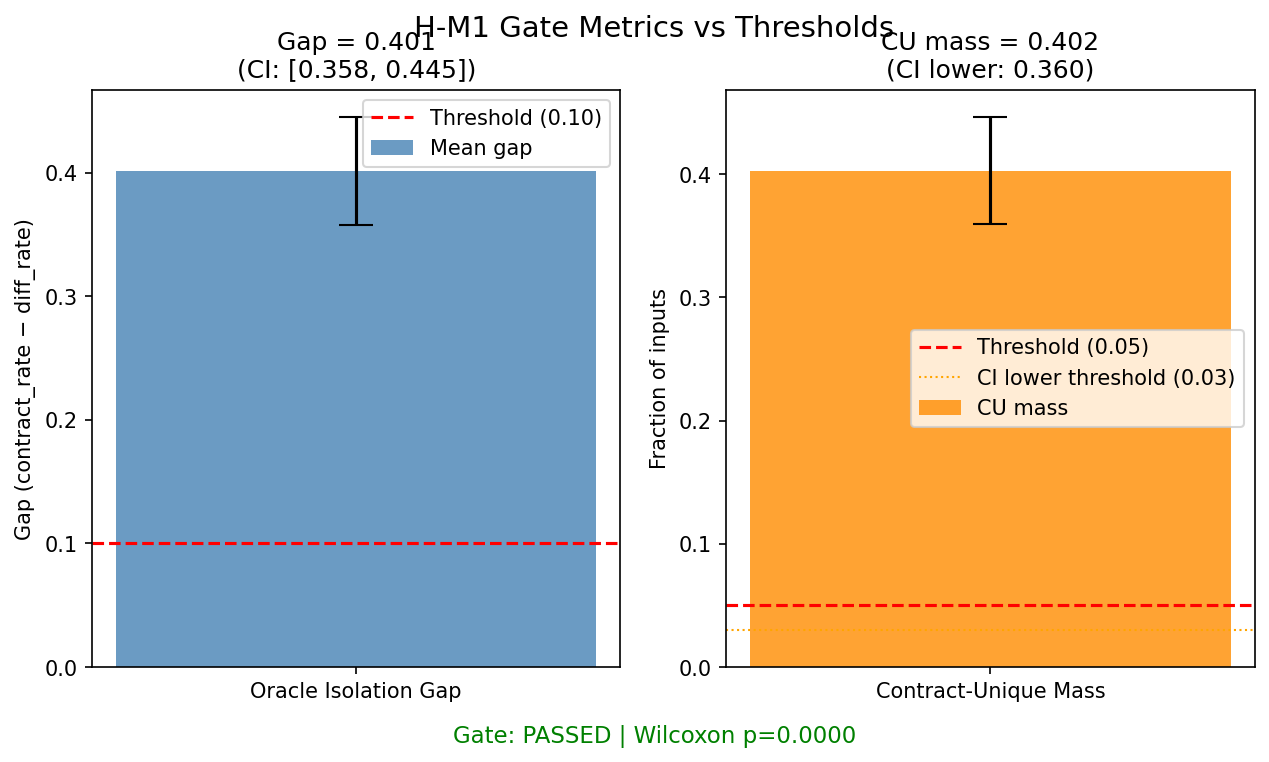
\includegraphics[width=\columnwidth]{figures/gate_metrics_comparison.png}
\caption{Gate metrics bar chart with 95\% CI}
\label{fig:gate_metrics_comparison}
\end{figure}

\textit{Figure 1: Oracle isolation gate metrics (oracle-isolation gap and contract-unique mass) with 95\% bootstrap CI.}

\begin{figure}[htbp]
\centering
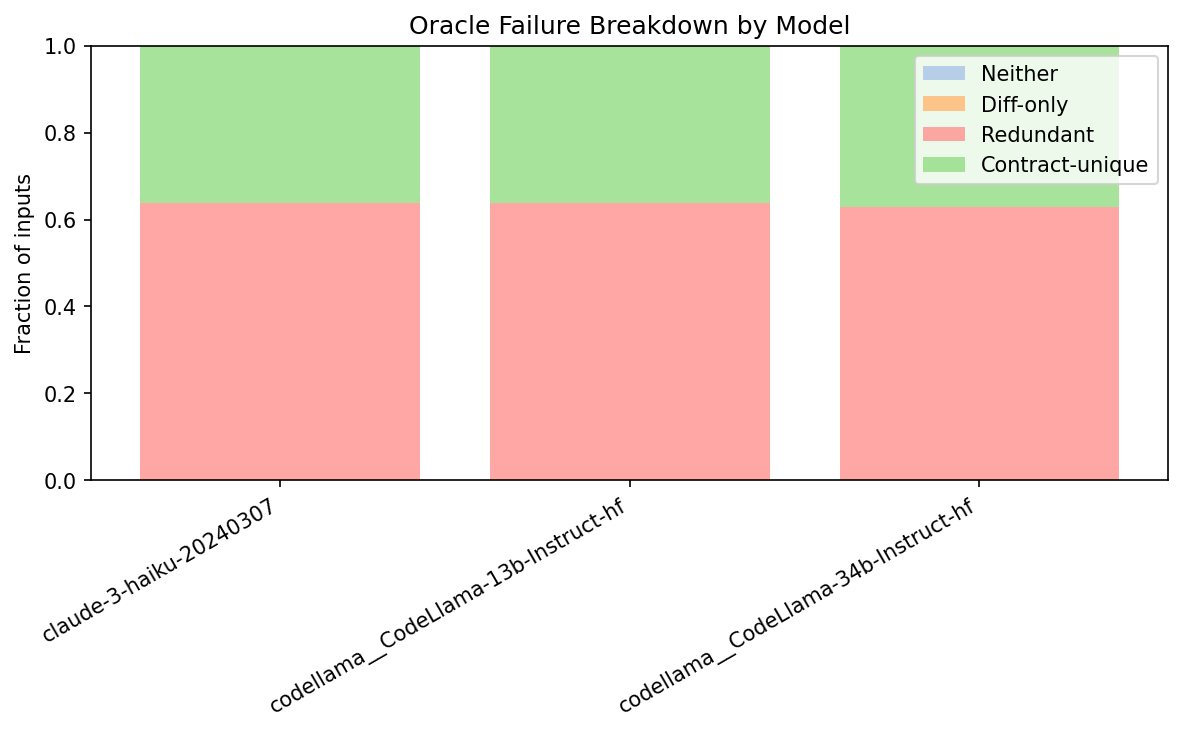
\includegraphics[width=\columnwidth]{figures/oracle_failure_breakdown.png}
\caption{Failure rate decomposition by category}
\label{fig:oracle_failure_breakdown}
\end{figure}

\textit{Figure 2: Differential vs. contract failure rate decomposition by model family.}

\begin{figure}[htbp]
\centering
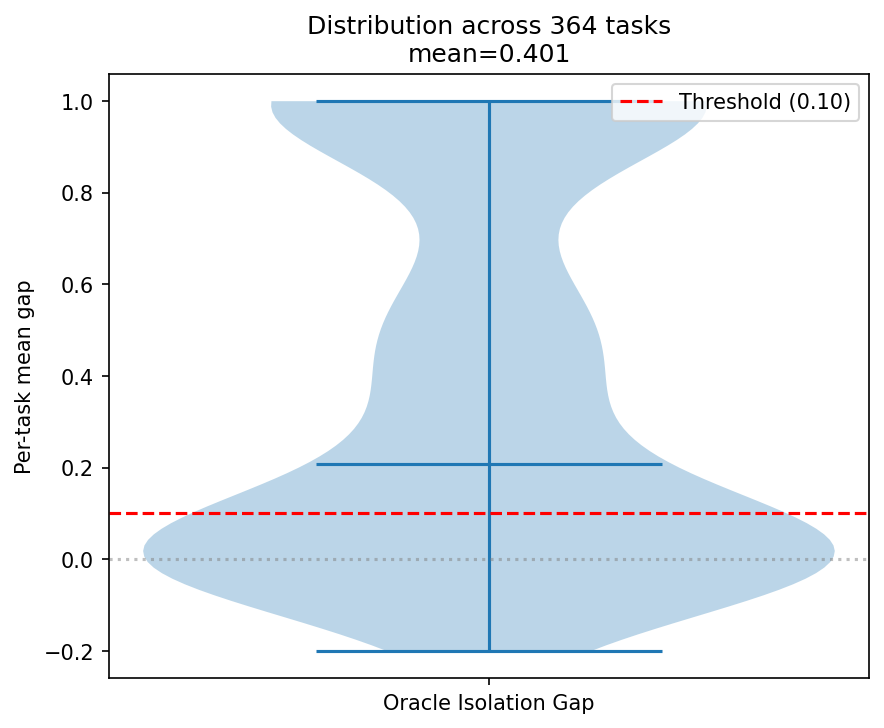
\includegraphics[width=\columnwidth]{figures/gap_distribution.png}
\caption{Violin plot of per-task oracle-isolation gap}
\label{fig:gap_distribution}
\end{figure}

\textit{Figure 3: Distribution of per-task oracle-isolation gaps across 364 tasks.}

\begin{figure}[htbp]
\centering
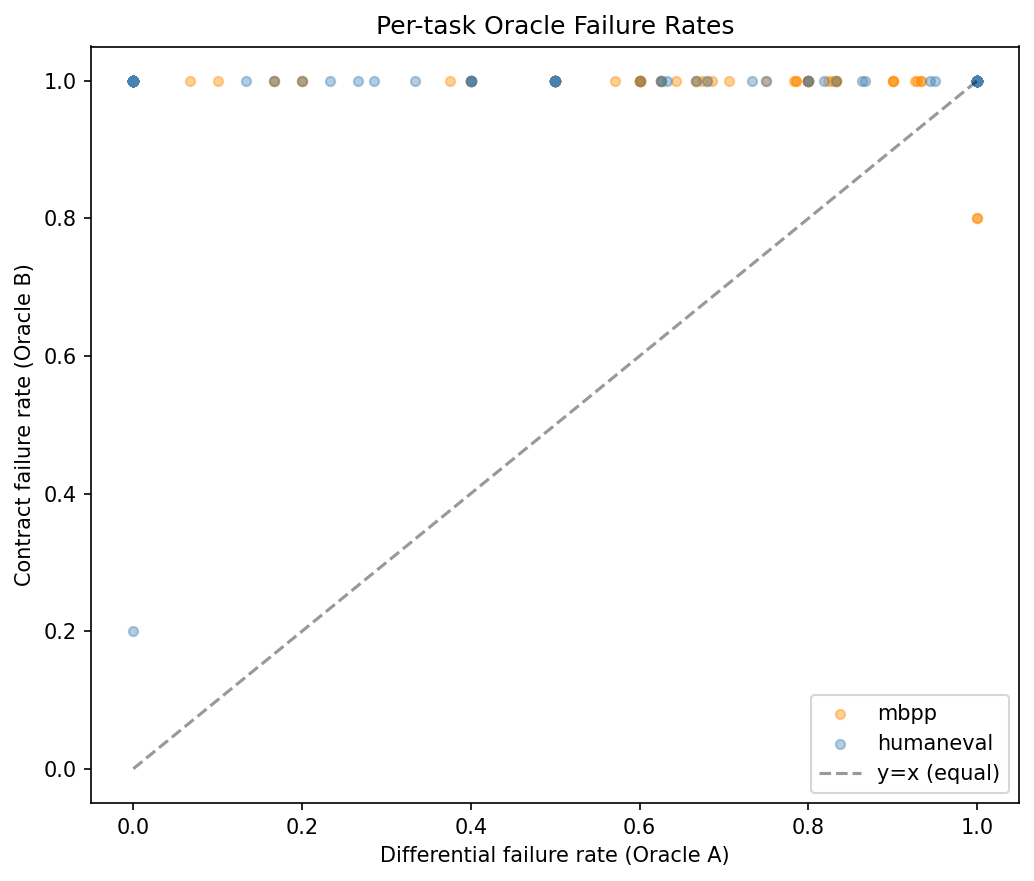
\includegraphics[width=\columnwidth]{figures/scatter_failure_rates.png}
\caption{Scatter: differential vs. contract failure rate per task}
\label{fig:scatter_failure_rates}
\end{figure}

\textit{Figure 4: Differential failure rate vs. contract failure rate per task on CVT inputs.}

\subsubsection{5.2 Adaptive PBT Contribution (RQ2)}

\textbf{Table 2: Adaptive PBT Gate Metrics (Experiment B)}

\begin{table}[htbp]
\centering
\resizebox{\columnwidth}{!}{%
\begin{tabular}{llll}
\toprule
Metric & Value & Threshold & Status \\
\midrule
Mean adaptive contribution & **0.0999** & > 0 & PASS \\
95\% CI & [0.065, 0.133] & CI lower > 0 & PASS \\
Wilcoxon p (one-sided) & **2.64e-22** & < 0.05 & PASS \\
Median adaptive contribution & 0.0908 & --- & --- \\
Tasks with positive contribution & 257 / 354 (72.6\%) & --- & --- \\
Joined evaluation triples & 17,226 & --- & --- \\
\bottomrule
\end{tabular}
}
\end{table}

Source: \texttt{h-m3/experiment\textbackslash \_results.json}

\textbf{Per-model adaptive contribution:}

\begin{table}[htbp]
\centering
\resizebox{\columnwidth}{!}{%
\begin{tabular}{llll}
\toprule
Model & Mean Contribution & Triples (n) & Positive Rate \\
\midrule
GPT-4o-mini & 0.1008 & 3,380 & 72.3\% \\
Claude-3-Haiku & 0.1013 & 3,516 & 73.1\% \\
DeepSeek-Coder-V2-Lite & 0.1033 & 3,388 & 72.9\% \\
CodeLlama-13B & 0.1027 & 3,472 & 73.1\% \\
CodeLlama-34B & 0.0993 & 3,470 & 73.0\% \\
**All models** & **0.0999** & **17,226** & **72.6\%** \\
\bottomrule
\end{tabular}
}
\end{table}

The adaptive contribution range across all 5 models is 0.099--0.103 (a spread of 0.004). This consistency --- across models spanning 7--34B parameters and open/closed architectures --- indicates the ~10 percentage point contribution is a property of the contract oracle and PBT input exploration strategy, not of model quality or architecture. Adaptive PBT and static oracle contribute independent detection layers.

\textbf{Task-type stratification:} HumanEval+ tasks show a mean adaptive contribution of 0.213 (n = 5,526 triples); MBPP+ tasks show 0.049 (n = 11,700 triples), indicating that HumanEval+ contracts admit substantially more additional violations through adaptive search.

The 354 tasks with Experiment B data (vs. 364 total) reflects 10 tasks excluded due to zero valid Experiment B triples from icontract-hypothesis incompatibility.

\begin{figure}[htbp]
\centering
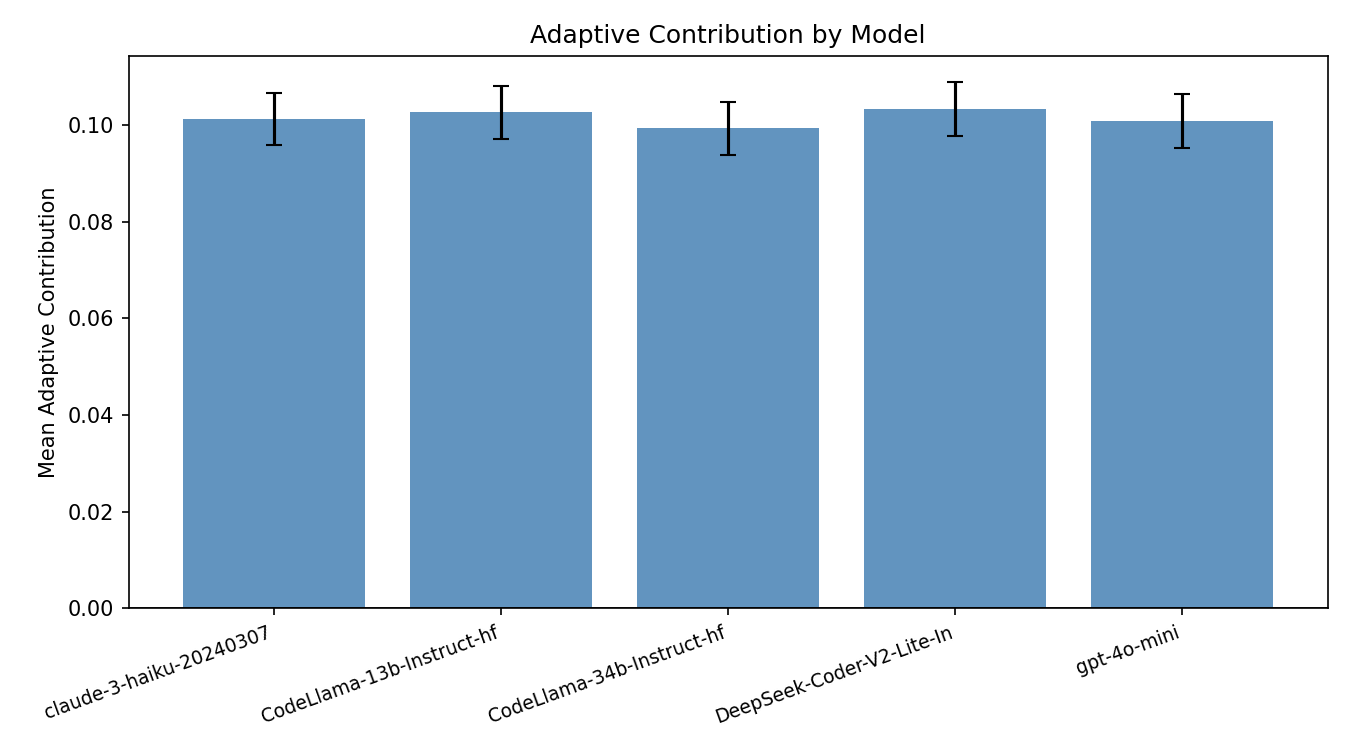
\includegraphics[width=\columnwidth]{figures/fig2_per_model.png}
\caption{Mean adaptive contribution by model}
\label{fig:fig2_per_model}
\end{figure}

\textit{Figure 5: Mean adaptive contribution by model family with standard error bars.}

\begin{figure}[htbp]
\centering
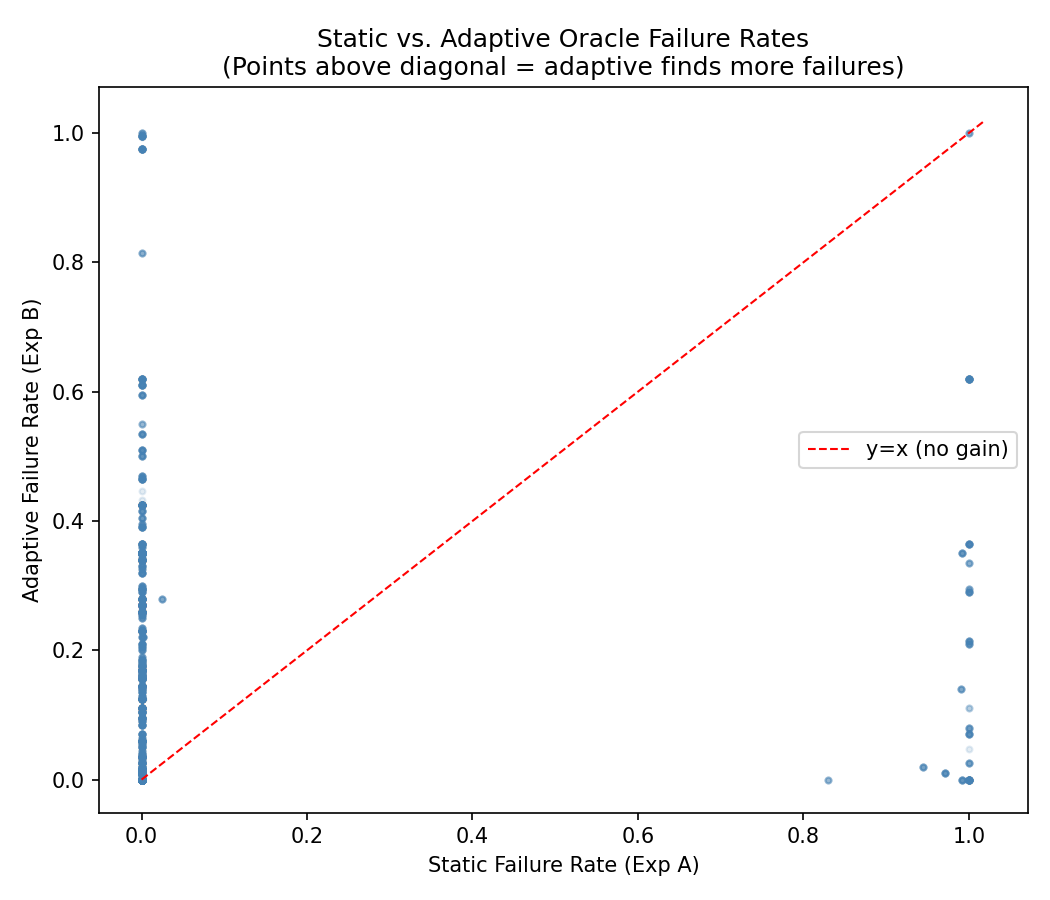
\includegraphics[width=\columnwidth]{figures/fig3_static_vs_adaptive.png}
\caption{Scatter: static CVT vs. adaptive PBT failure rate per triple}
\label{fig:fig3_static_vs_adaptive}
\end{figure}

\textit{Figure 6: Static CVT failure rate vs. adaptive PBT failure rate per (task, model, program) triple.}

\begin{figure}[htbp]
\centering
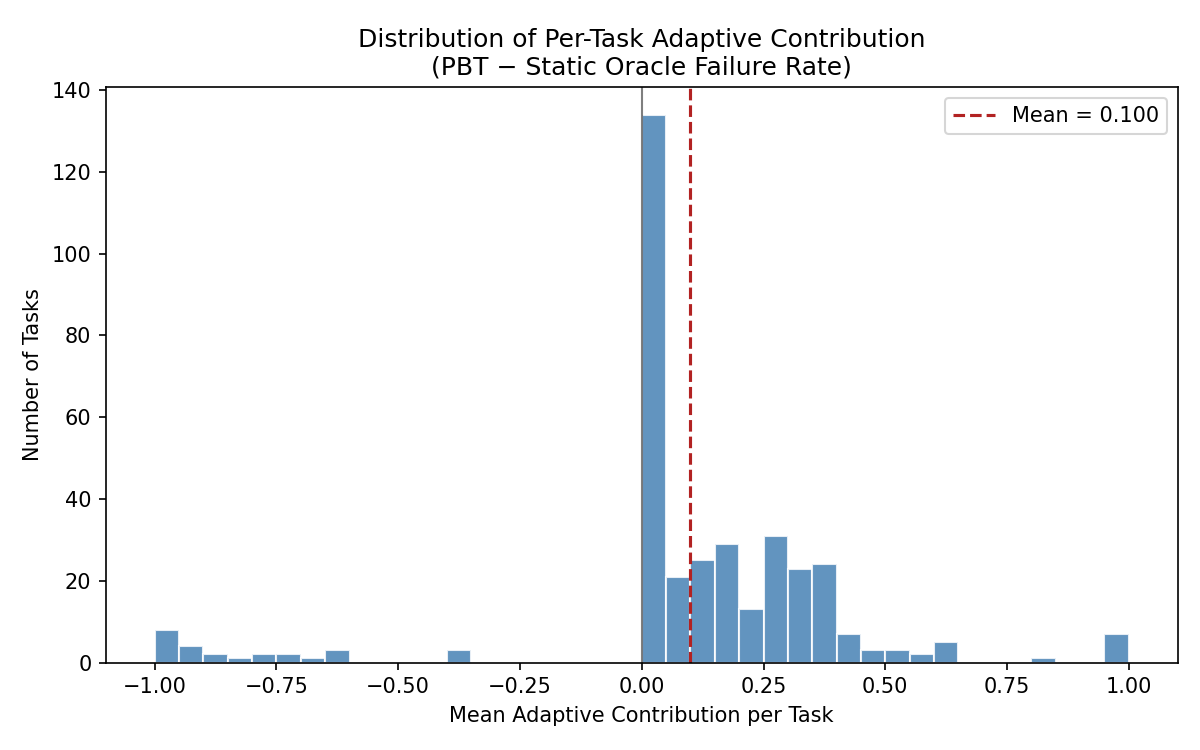
\includegraphics[width=\columnwidth]{figures/fig1_task_mean_distribution.png}
\caption{Distribution of per-task mean adaptive contribution}
\label{fig:fig1_task_mean_distribution}
\end{figure}

\textit{Figure 7: Histogram of per-task mean adaptive contribution across 354 tasks.}

\begin{figure}[htbp]
\centering
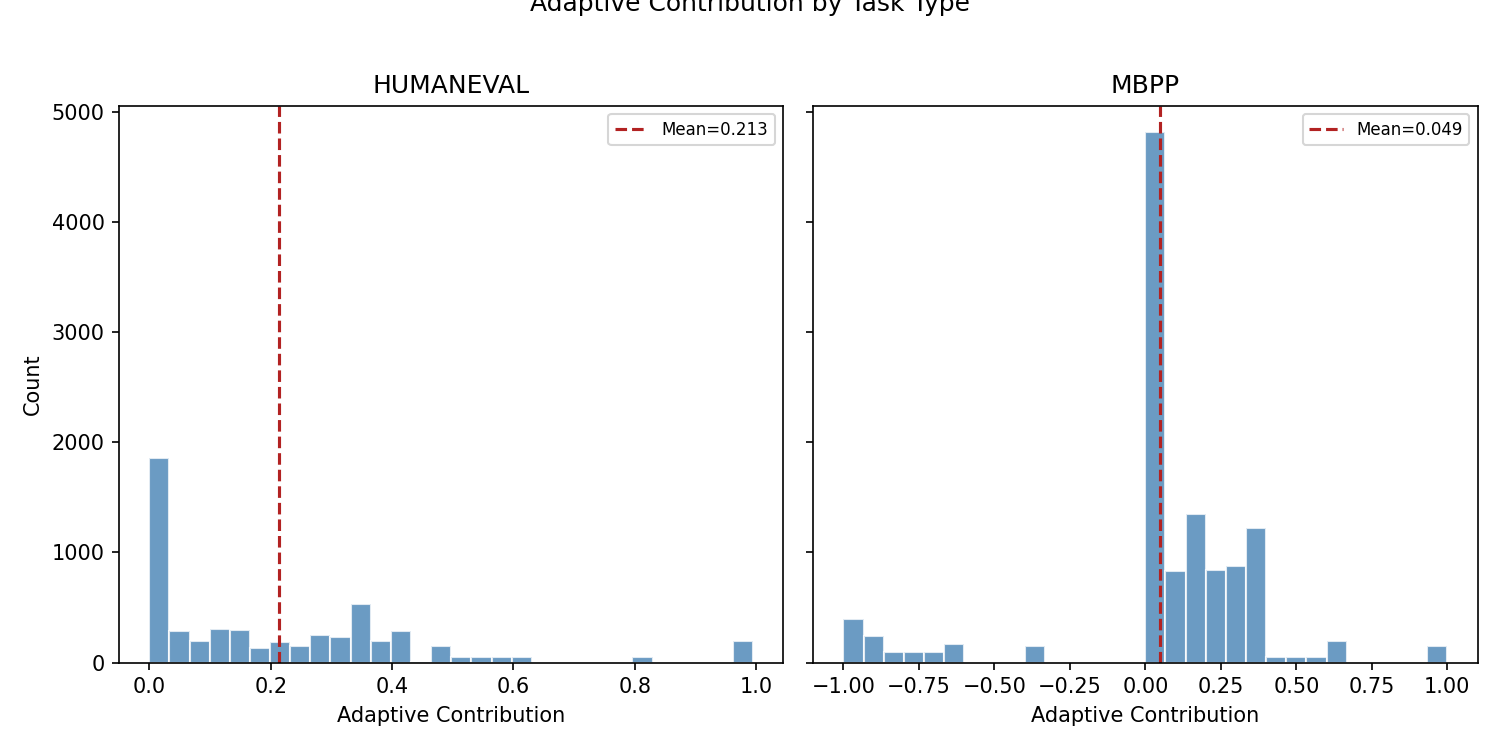
\includegraphics[width=\columnwidth]{figures/fig4_by_task_type.png}
\caption{Adaptive contribution by task type}
\label{fig:fig4_by_task_type}
\end{figure}

\textit{Figure 8: Adaptive contribution distribution by task type (HumanEval+ vs. MBPP+).}

\subsubsection{5.3 Contract Richness Correlation (RQ3)}

\textbf{Table 3: Richness-Gap Correlation (Experiment C)}

\begin{table}[htbp]
\centering
\resizebox{\columnwidth}{!}{%
\begin{tabular}{llll}
\toprule
Metric & Value & Threshold & Status \\
\midrule
Spearman $\rho$ (exact permutation) & 0.136 & $\geq$ 0.30 & BELOW THRESHOLD \\
p-value (exact permutation) & 5.30e-03 & < 0.05 & Significant \\
95\% CI & [0.034, 0.235] & --- & --- \\
Kruskal-Wallis H & 11.22 & --- & --- \\
Kruskal-Wallis p & 0.0106 & --- & Significant \\
\bottomrule
\end{tabular}
}
\end{table}

Source: \texttt{h-m2/experiment\textbackslash \_results.json}

\textbf{Per-tier oracle-isolation gap:}

\begin{table}[htbp]
\centering
\resizebox{\columnwidth}{!}{%
\begin{tabular}{llll}
\toprule
Tier & Label & Mean Oracle Gap & Tasks (n) \\
\midrule
1 & Simple (basic comparisons) & 0.339 & 178 (48.9\%) \\
2 & Structural (BoolOp chaining) & **0.523** & 40 (11.0\%) \\
3 & Relational (any/all quantification) & 0.436 & 117 (32.1\%) \\
4 & Compound & 0.473 & 29 (8.0\%) \\
\bottomrule
\end{tabular}
}
\end{table}

The Spearman $\rho$ = 0.136 is statistically significant (p = 0.005, exact permutation) and positive in direction, but falls below the $\rho \geq$ 0.30 threshold. The tier gradient is non-monotonic: Tier 2 shows a higher mean gap (0.523) than both Tier 3 (0.436) and Tier 4 (0.473). This ordering likely reflects the nature of ContractEval's contracts: Tier 2 BoolOp contracts function primarily as input validity checks (preconditions that chain boolean conditions), which fire reliably on CVT inputs designed to violate preconditions.

The pattern is consistent with a threshold effect: the presence of any formal contract assertion --- regardless of AST complexity --- creates a substantial oracle-isolation gap (~0.40 across all tiers), while the additional contribution of greater contract complexity is weak and non-monotonic. Between-tier group differences are statistically detectable (Kruskal-Wallis p = 0.011), but the continuous richness-gap relationship is weak.

\begin{figure}[htbp]
\centering
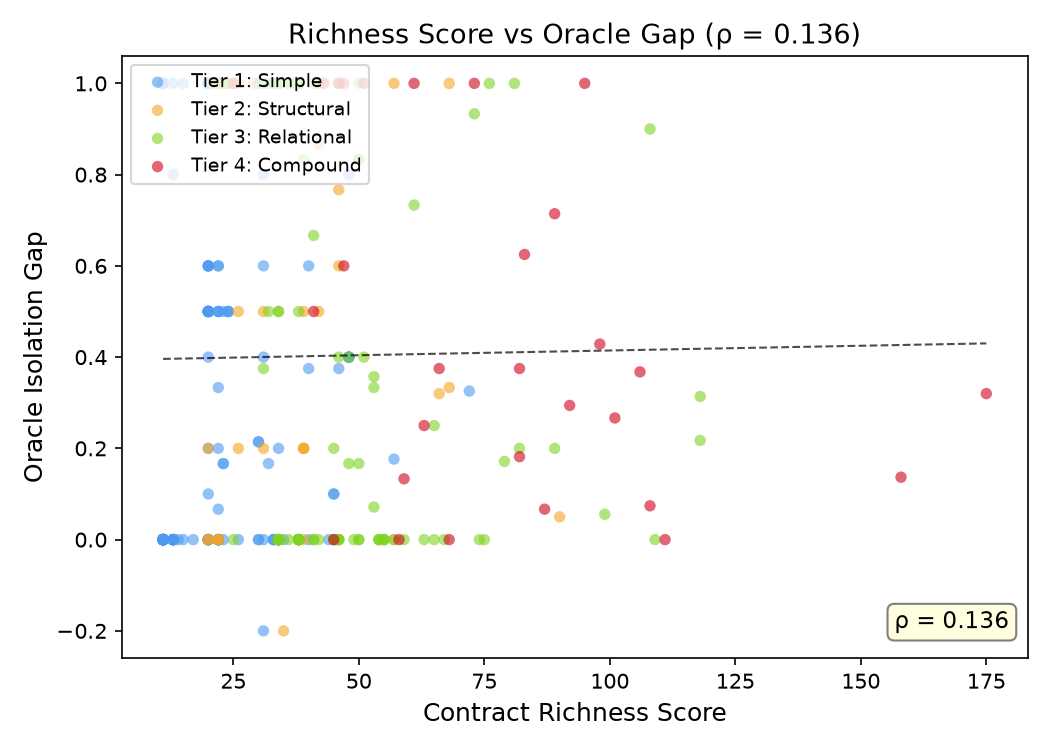
\includegraphics[width=\columnwidth]{figures/figure_scatter.png}
\caption{Scatter: richness score vs. oracle gap per task}
\label{fig:figure_scatter}
\end{figure}

\textit{Figure 9: AST-based richness score vs. oracle-isolation gap per task.}

\begin{figure}[htbp]
\centering
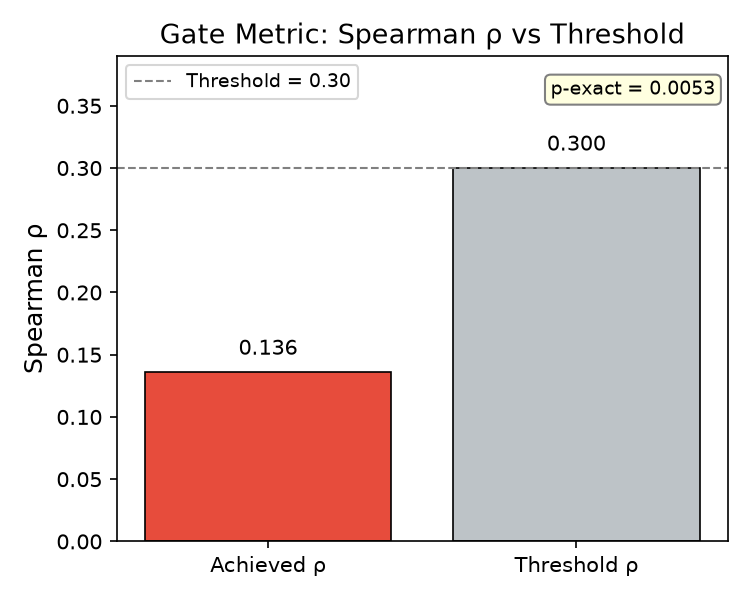
\includegraphics[width=\columnwidth]{figures/figure_gate_metrics.png}
\caption{Bar chart of oracle-isolation gap by richness tier}
\label{fig:figure_gate_metrics}
\end{figure}

\textit{Figure 10: Mean oracle-isolation gap by contract richness tier.}

\subsubsection{5.4 Cross-Model Analysis (RQ4)}

The following table notes that FAIL entries reflect structural statistical constraints (n = 5 models structurally precludes achieving p < 0.05 for $\tau$ = 0.40 under exact permutation test), not hypothesis failures. The $\Delta R^2$ = 0.004 and cross-model gap = 0.007 are genuine null findings.

\textbf{Table 4: Cross-Model Analysis Gate Metrics (Experiment D)}

\begin{table}[htbp]
\centering
\resizebox{\columnwidth}{!}{%
\begin{tabular}{llll}
\toprule
Metric & Value & Threshold & Status \\
\midrule
Kendall $\tau$ & 0.40 & $\leq$ 0.60 & PASS \\
Permutation p (exact, two-sided) & 0.4833 & < 0.05 & FAIL (structural: n=5) \\
Partial $\Delta R^2$ (model identity) & 0.0044 & $\geq$ 0.10 & FAIL (null finding) \\
Cross-model gap (task-controlled) & 0.0069 & $\geq$ 0.10 & FAIL (null finding) \\
Cross-model gap 95\% CI & [0.0047, 0.0093] & --- & --- \\
$R^{2}_full$ & 0.5005 & --- & --- \\
$R^{2}_reduced$ & 0.4961 & --- & --- \\
n model-task pairs & 1,815 & --- & --- \\
\bottomrule
\end{tabular}
}
\end{table}

Source: \texttt{h-m4/results/h\textbackslash \_m4\textbackslash \_results.json}

\textbf{Model rankings by contract-satisfaction rate:} GPT-4o-mini > DeepSeek-Coder-V2-Lite > CodeLlama-34B > CodeLlama-13B > Claude-3-Haiku.

*\textit{Model rankings by pass@1}:** DeepSeek-Coder-V2-Lite > GPT-4o-mini > Claude-3-Haiku > CodeLlama-34B > CodeLlama-13B.

Kendall $\tau$ = 0.40 satisfies the $\leq$ 0.60 threshold, showing moderate non-monotonicity between rankings (e.g., GPT-4o-mini ranks 1st on contract satisfaction but 2nd on pass@1\textit{; Claude-3-Haiku ranks last on contract satisfaction but 3rd on pass@1}). However, p = 0.4833 reflects a structural constraint: with n = 5 models, the exact permutation test produces a null distribution over 14,400 pairings-mode permutations, and the minimum achievable two-sided p is approximately 0.017 (at |$\tau |$ = 1.0 only). For $\tau$ = 0.40, p $\approx$ 0.48 is the correct result under $H_0$.

The $\Delta R^2$ = 0.004 is interpretable independently as a genuine null: model family identity adds negligible explanatory power beyond pass@1* and log(model size) in this 5-model set. The task-controlled residual gap of 0.007 (approximately $15\times$ below the 0.10 threshold) indicates between-task variance dominates over between-model variance in this evaluation scope.

Subgroup analysis: HumanEval+ $\tau$ = 0.20 ($\Delta R^2 = -0.009)$; MBPP+ $\tau$ = 0.40 ($\Delta R^2 = -0.003)$. Both subgroups confirm near-zero model identity contribution.

\begin{figure}[htbp]
\centering
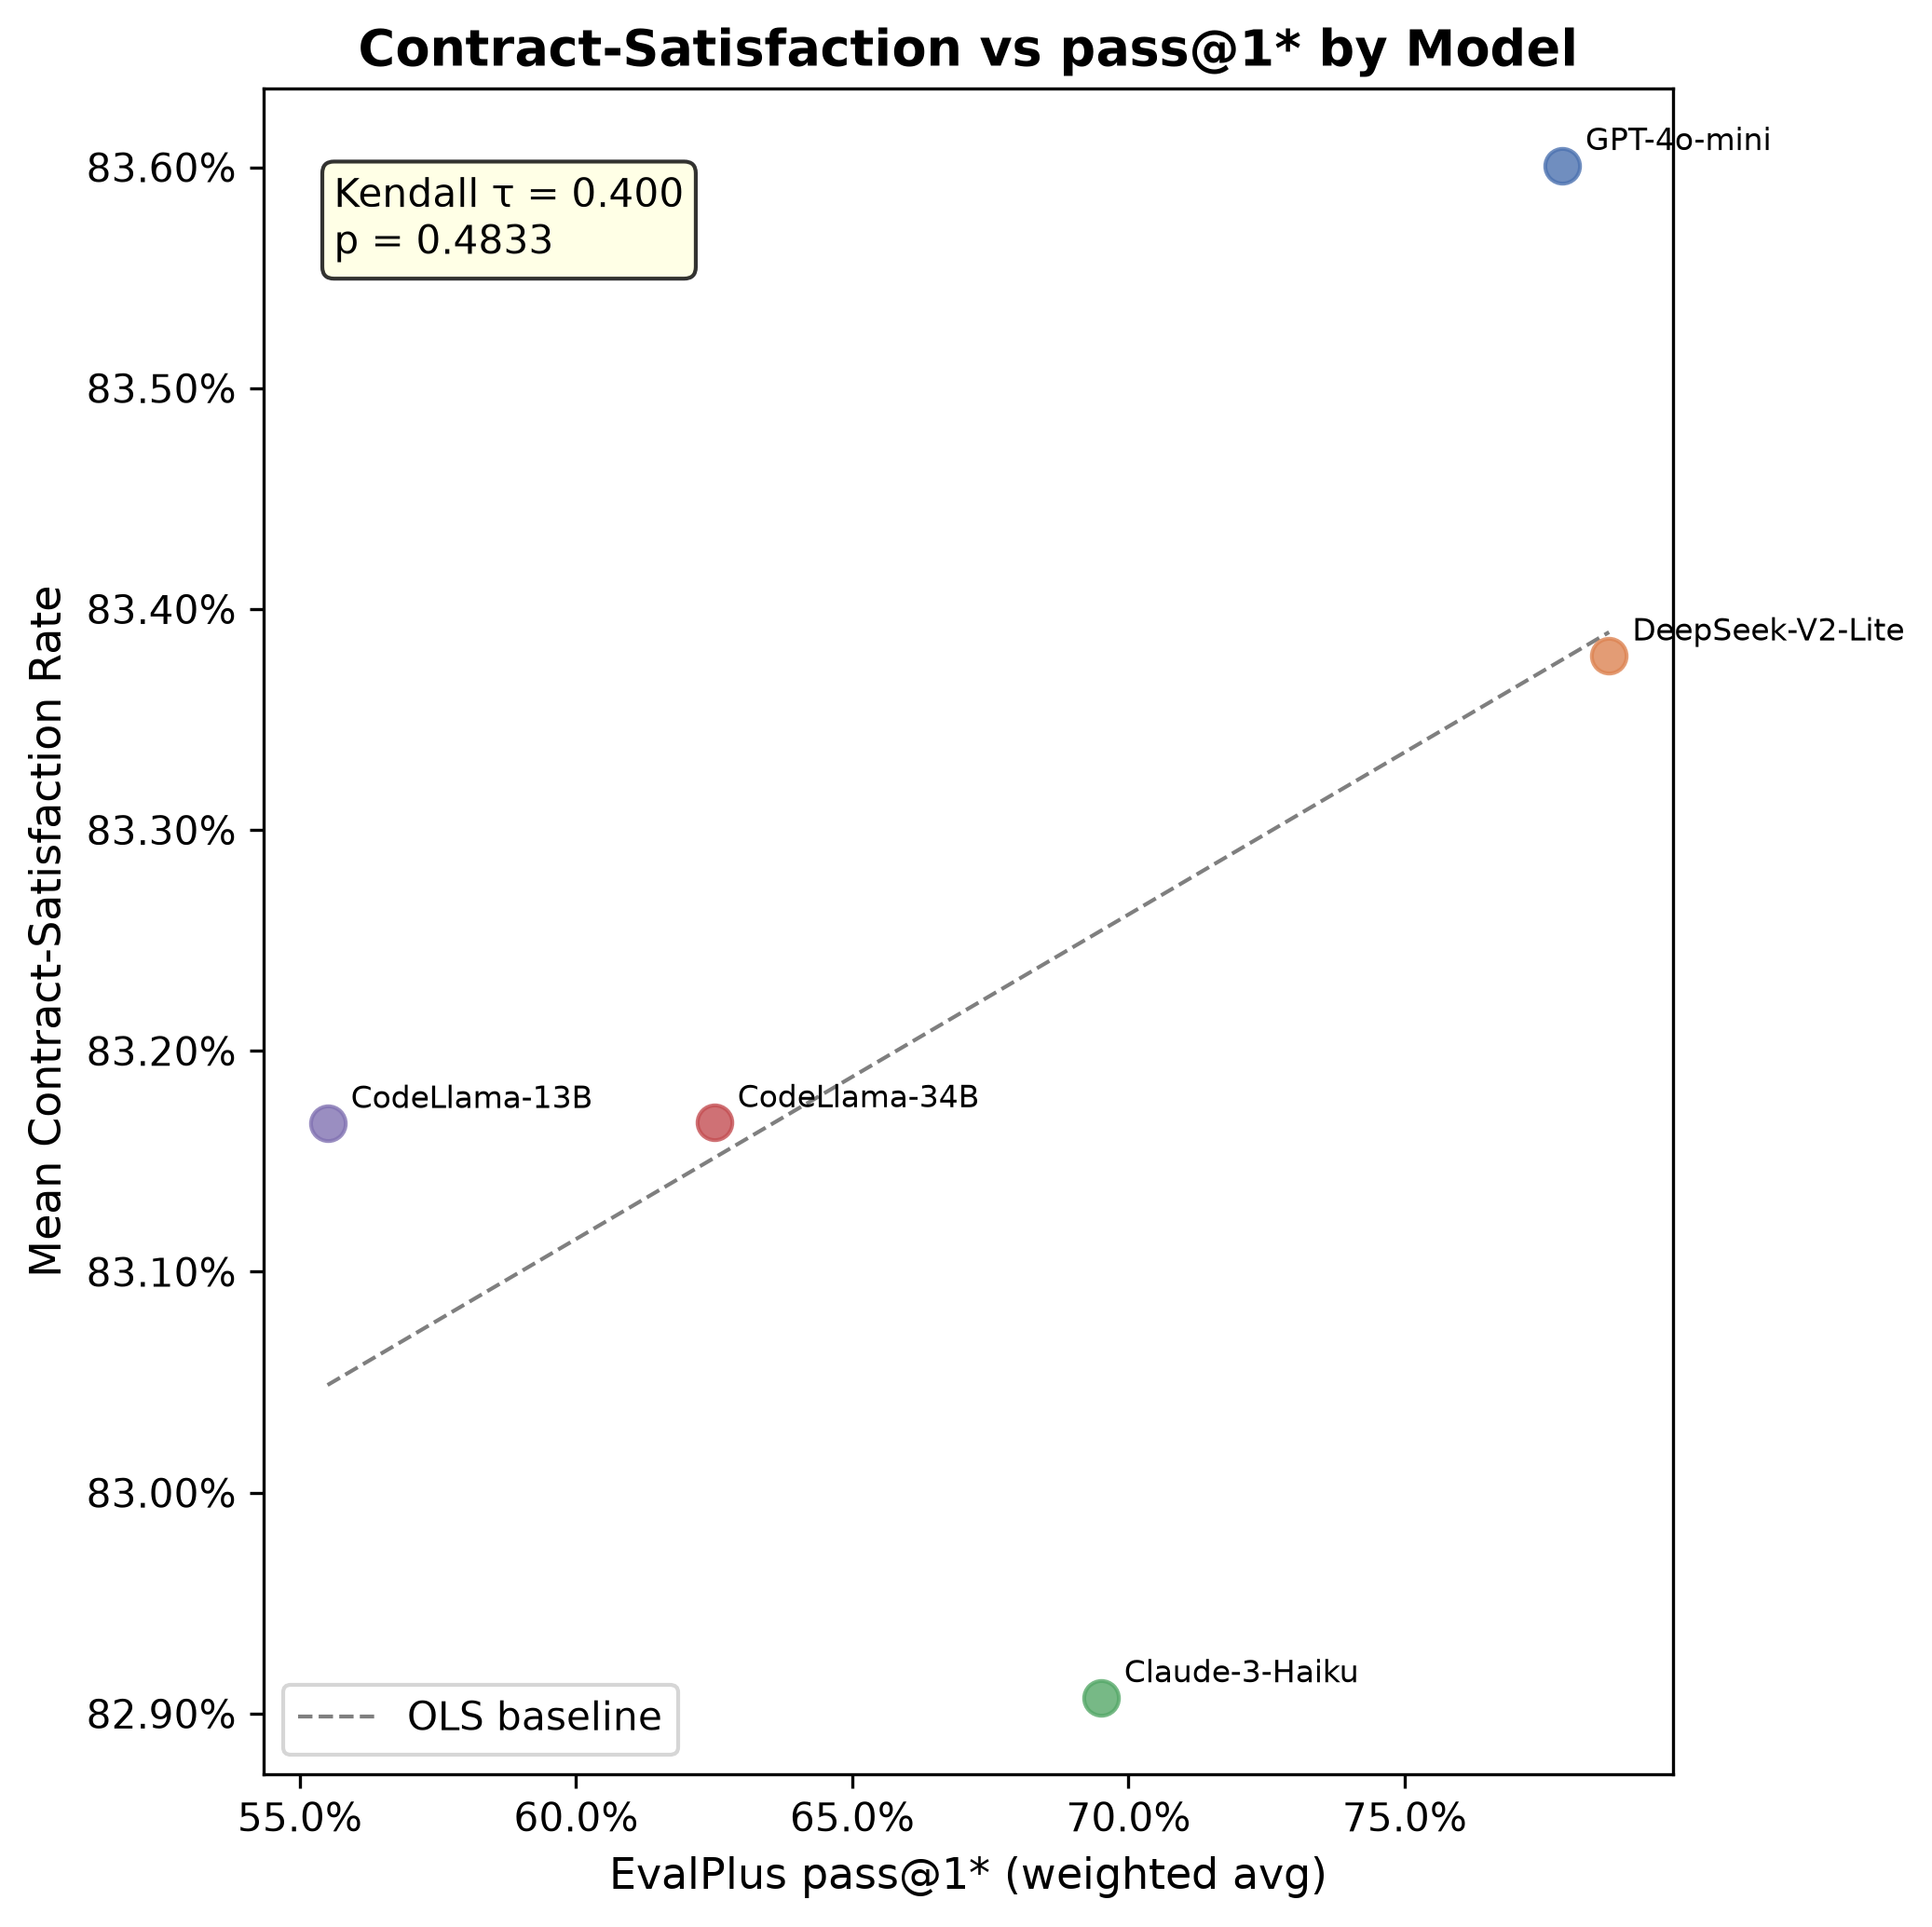
\includegraphics[width=\columnwidth]{figures/ranking_scatter.png}
\caption{Contract satisfaction rate vs. pass@1* scatter}
\label{fig:ranking_scatter}
\end{figure}

\textit{Figure 11: Contract-satisfaction rate vs. pass@1} for 5 model families.*

\begin{figure}[htbp]
\centering
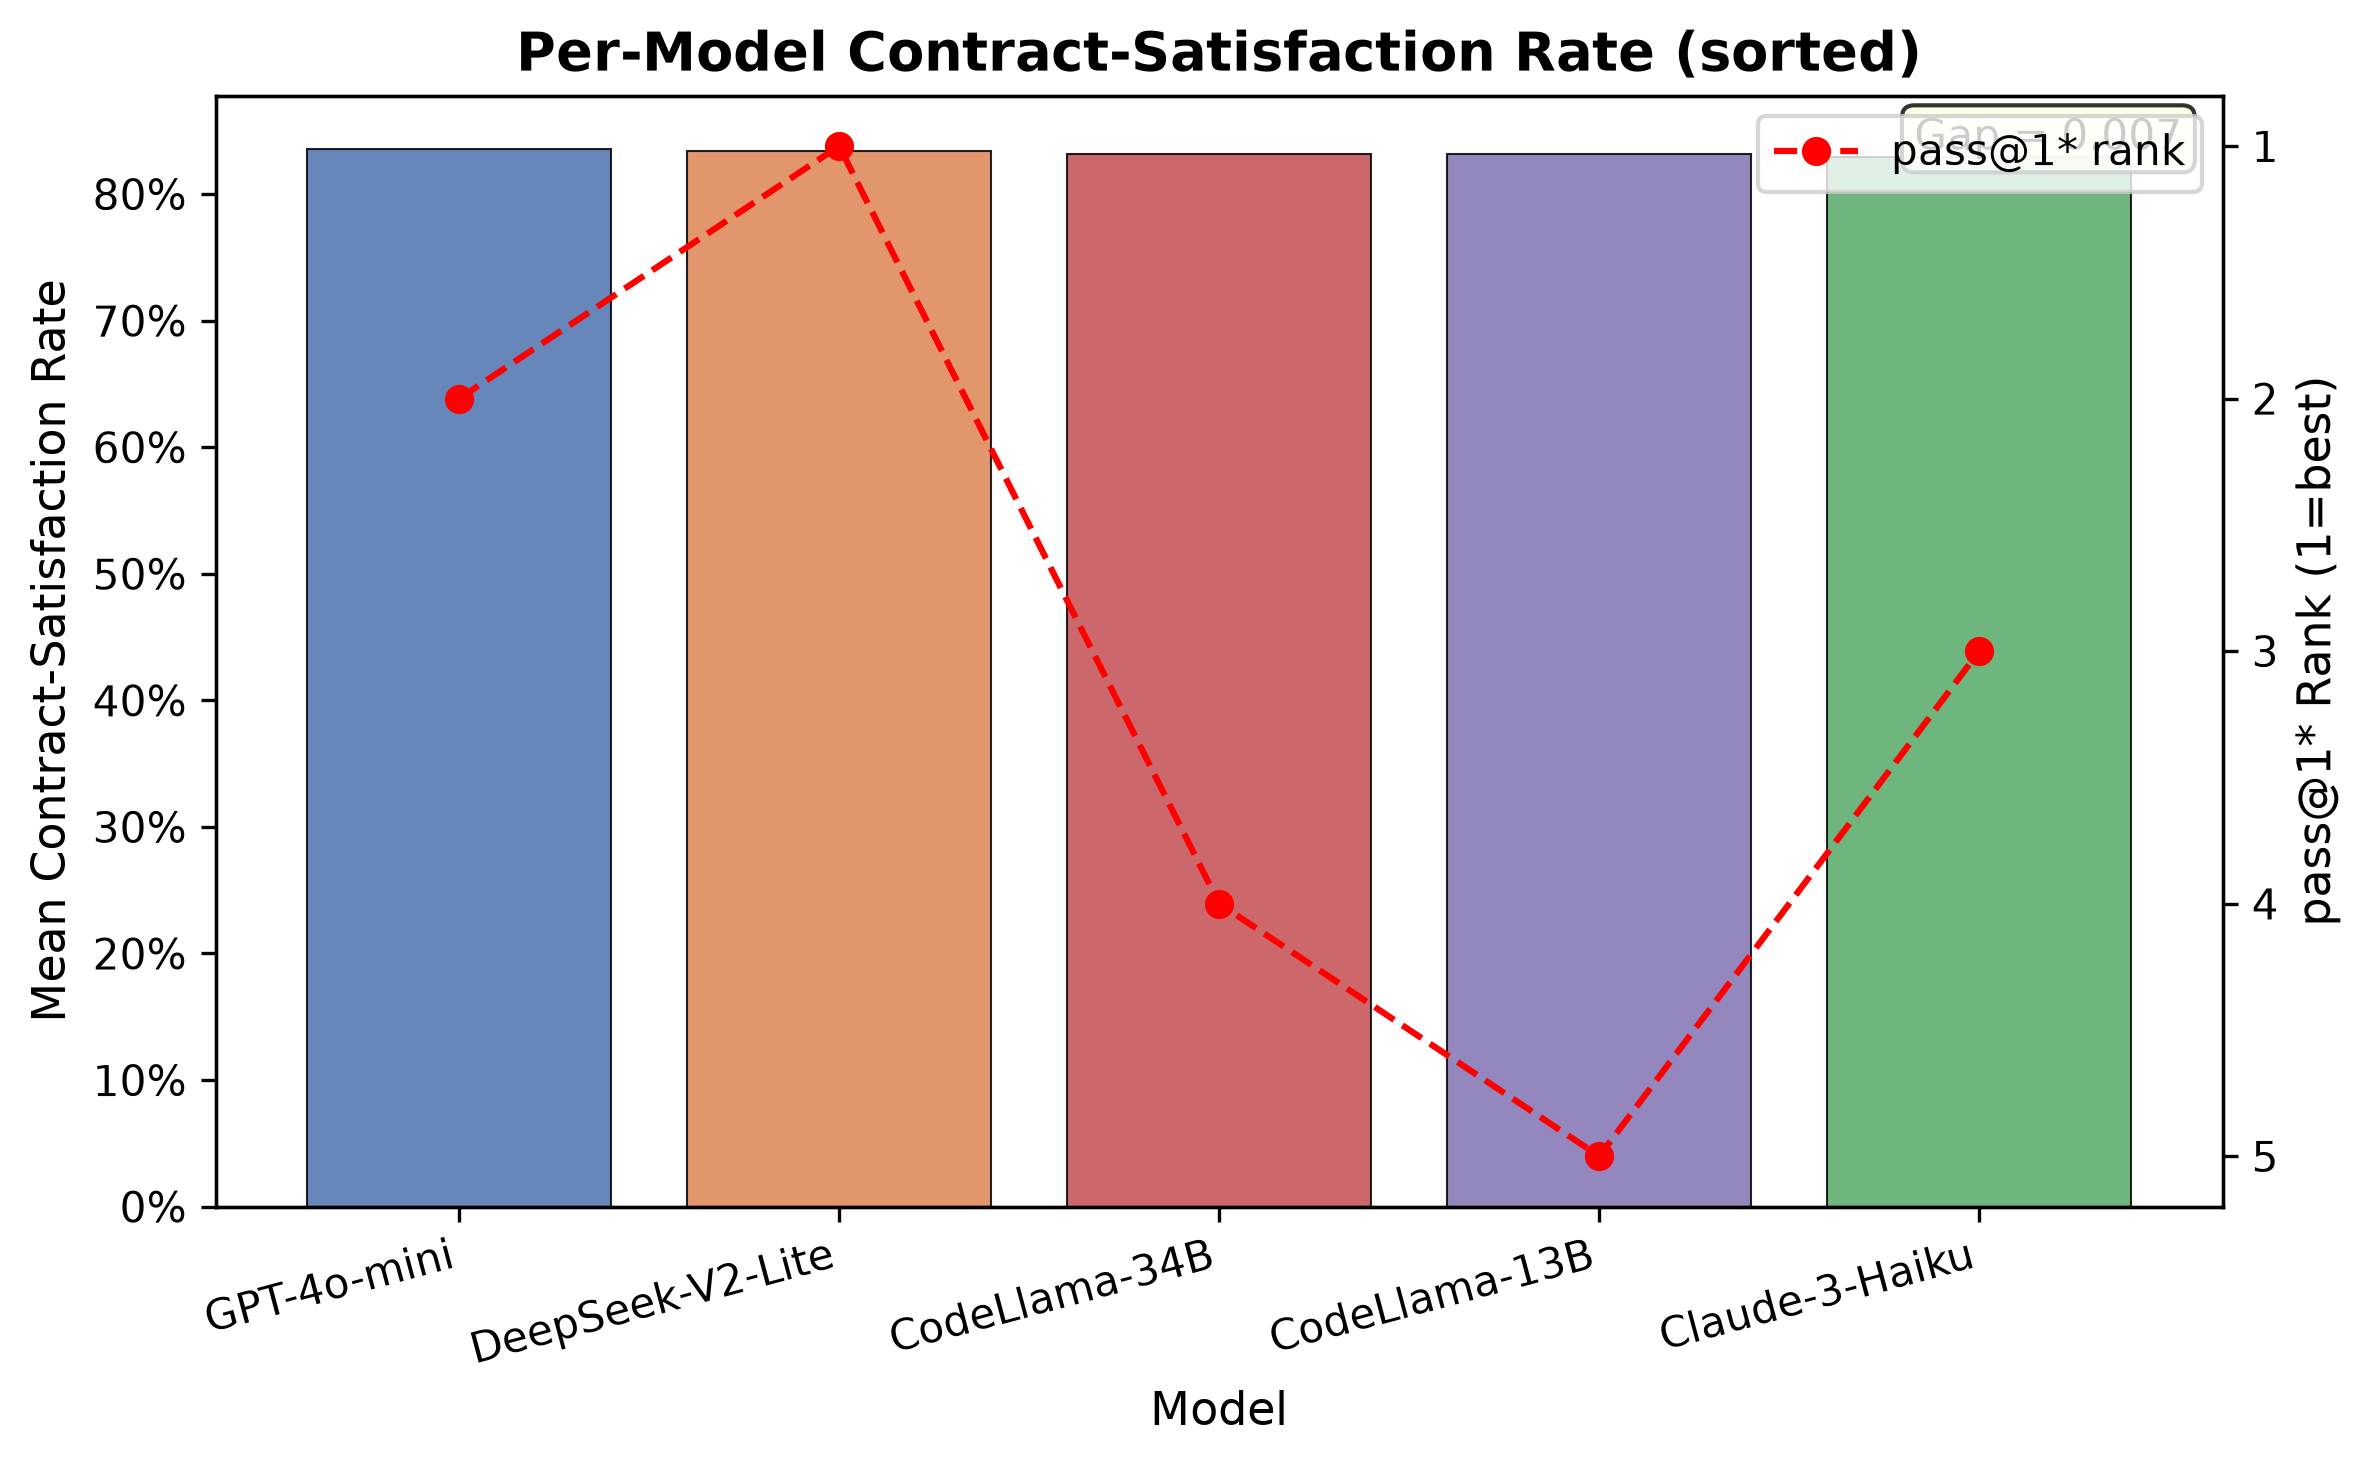
\includegraphics[width=\columnwidth]{figures/cross_model_bar.png}
\caption{Per-model mean contract satisfaction rate}
\label{fig:cross_model_bar}
\end{figure}

\textit{Figure 12: Per-model mean contract-satisfaction rate.}

\begin{figure}[htbp]
\centering
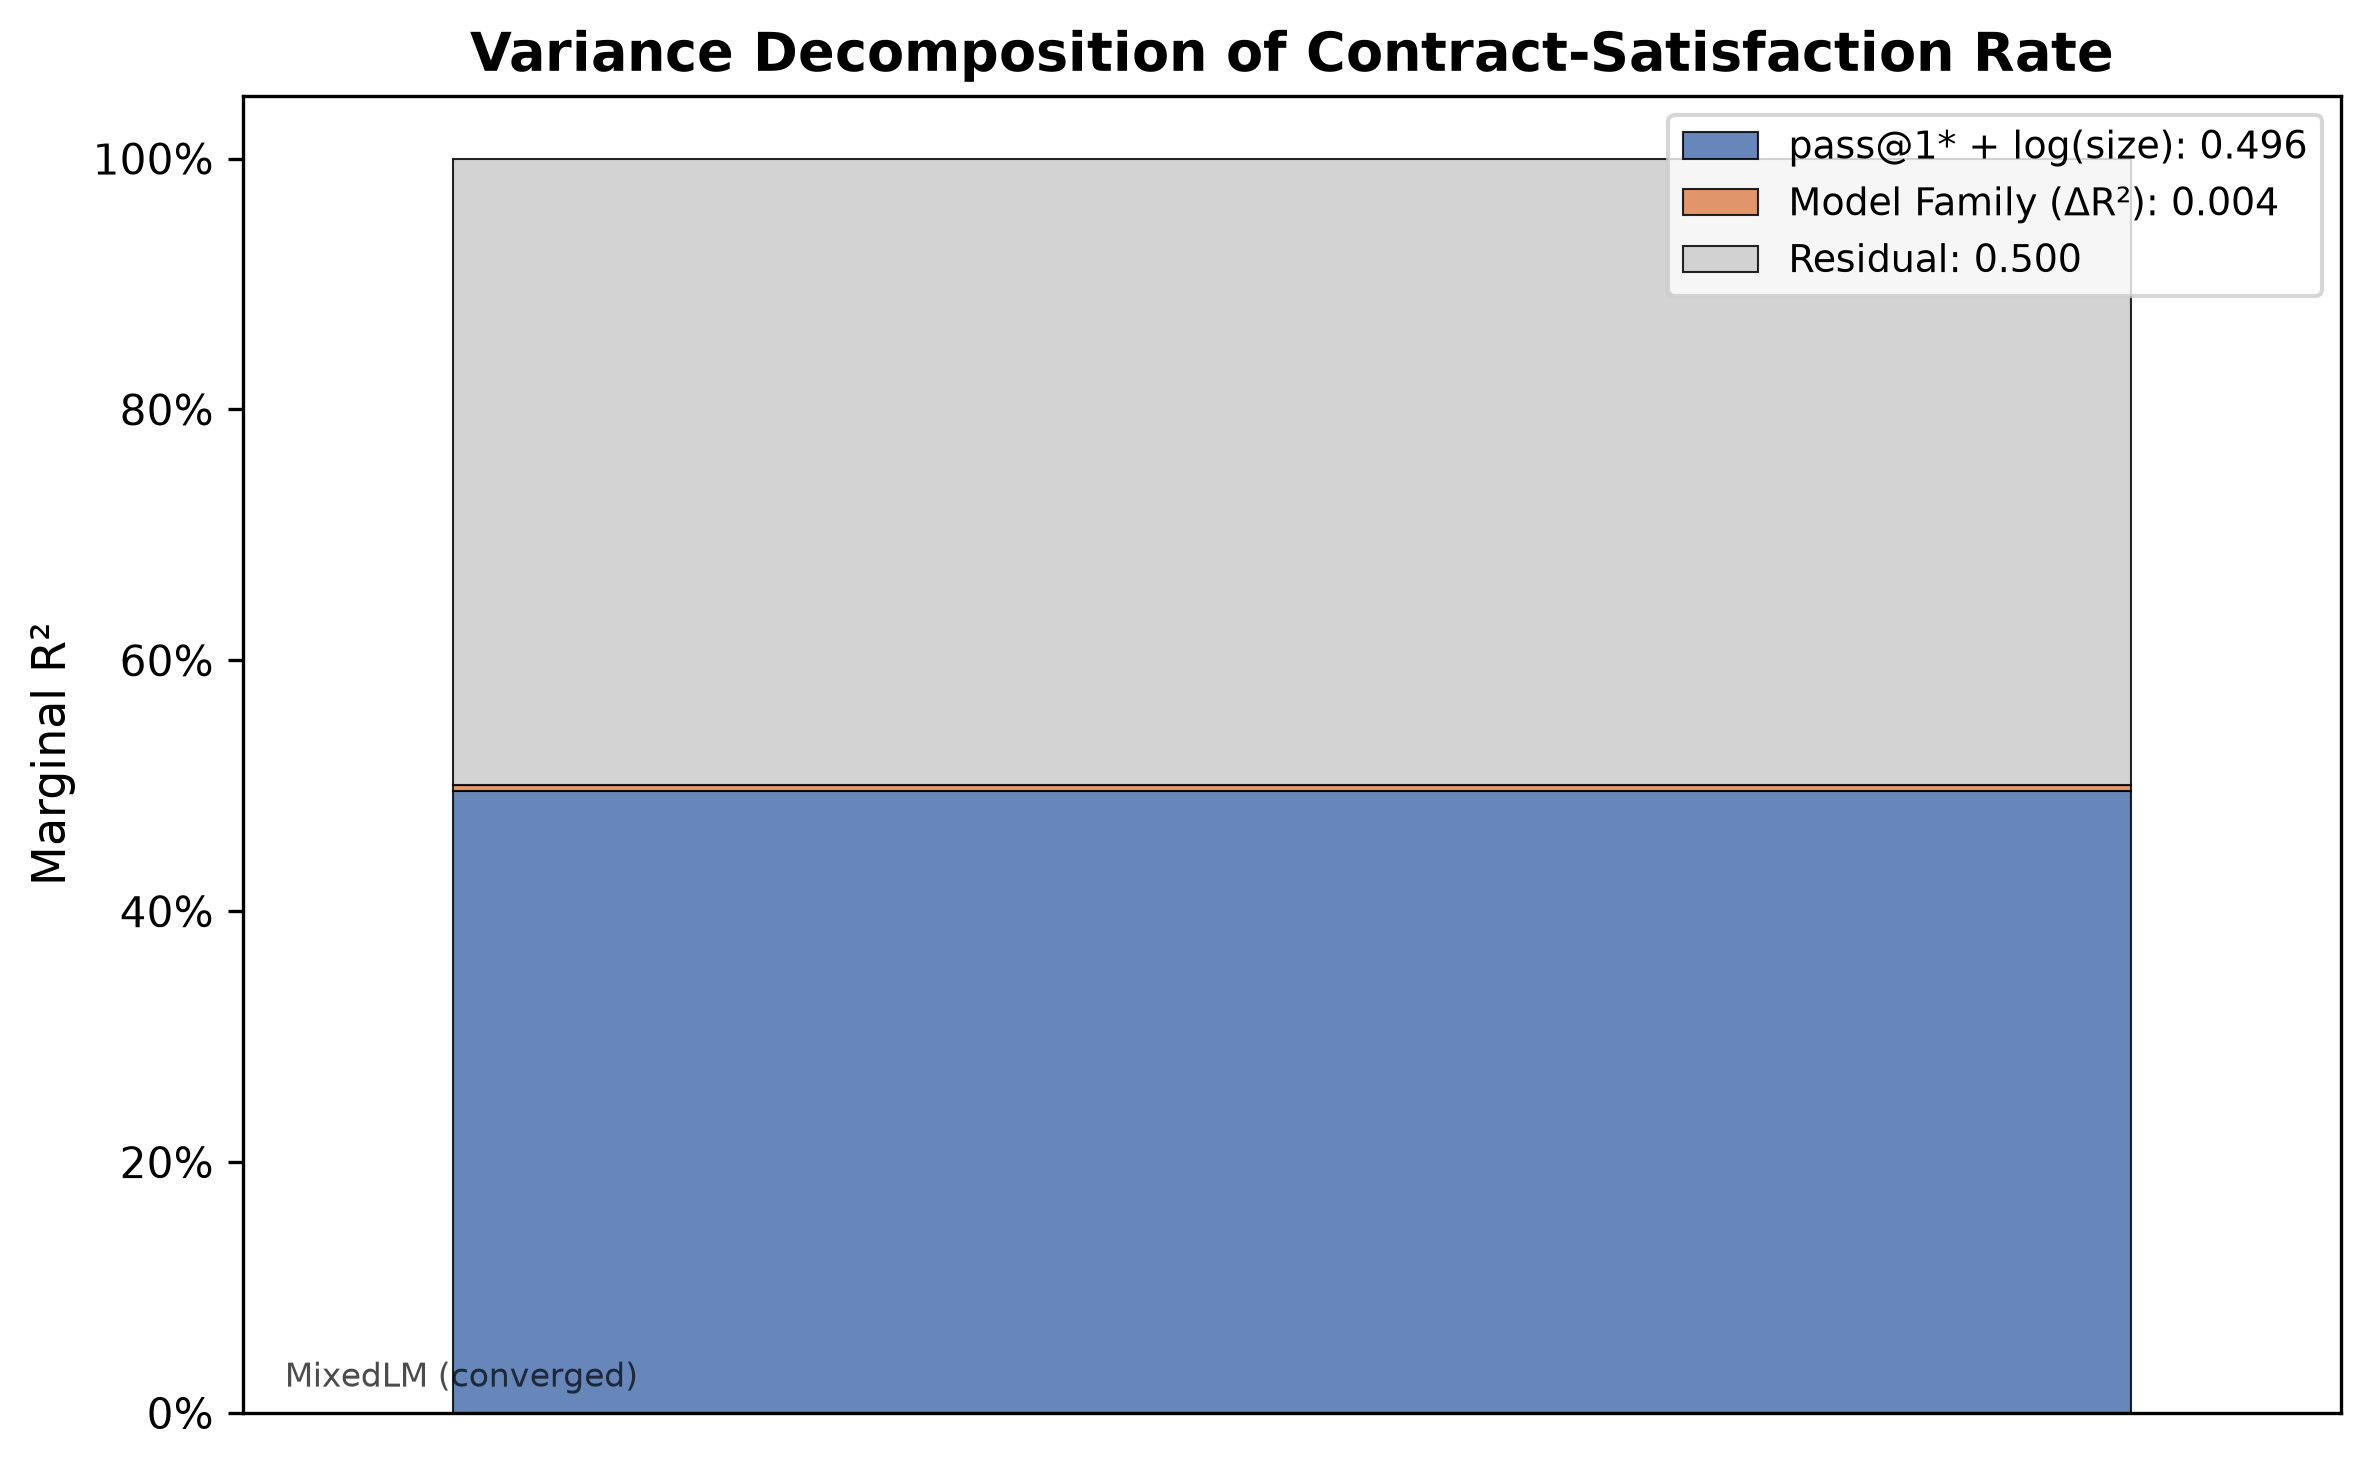
\includegraphics[width=\columnwidth]{figures/r2_decomposition.png}
\caption{Variance decomposition}
\label{fig:r2_decomposition}
\end{figure}

\textit{Figure 13: Variance decomposition: $R^2$ contributions from pass@1}, log(size), and model identity.*

\subsubsection{5.5 Summary Across Hypotheses}

\begin{table*}[htbp]
\centering
\resizebox{\dimexpr 2\columnwidth+\columnsep\relax}{!}{%
\begin{tabular}{lllll}
\toprule
Sub-hypothesis & Gate & Result & Key Metric & Status \\
\midrule
h-e1: Gap exists (364 tasks) & MUST\_WORK & PASS & 228/364 tasks (62.6\%) show $\geq 1$ violation; oracle precheck: 364/364 & Validated \\
h-m1: Oracle gap $\geq$ 0.10 & MUST\_WORK & PASS & Gap = 0.4012; CU mass = 0.4023; p = 5.88e-38 & Validated \\
h-m3: Adaptive adds > 0 & MUST\_WORK & PASS & 0.0999; p = 2.64e-22; uniform across 5 models & Validated \\
h-m2: Richness $\rho \geq$ 0.30 & SHOULD\_WORK & FAIL & $\rho$ = 0.136; threshold effect observed & Negative result \\
h-m4: Cross-model orthogonality & SHOULD\_WORK & PARTIAL & $\tau$ = 0.40 (criterion met); p = 0.48 (structural); $\Delta R^2$ null & Underpowered / null \\
\bottomrule
\end{tabular}
}
\end{table*}

All three MUST\_WORK gate criteria are satisfied. Both SHOULD\_WORK failures are recorded as principled negative results or structural limitations.

